\documentclass[review,authoryear]{elsarticle} 

\usepackage{lineno}
%% define acronyms here
% define packages here
\usepackage{acronym} %% using acronyms
\usepackage{amsmath}
\usepackage{amssymb}
\usepackage{array} 
\usepackage{booktabs}
\usepackage{caption}
\usepackage{fancyvrb}
\usepackage{filecontents}
\usepackage{float}% [H] option for figures
\usepackage{graphicx}
\usepackage{hyperref}
\usepackage[acronym]{glossaries}% put after hyperref package
\usepackage{imakeidx}
\usepackage{lineno}
\usepackage{listings}
% \usepackage[round,sort]{natbib}
\usepackage{paralist}
\usepackage{pdflscape}
\usepackage{siunitx}
\usepackage{tabu}
\usepackage{textcomp}
\usepackage{upquote}
\usepackage{xcolor}
\usepackage{url}


% define verbatim formulas
\newcommand{\vv}[1]{{\tt #1}}


% define caption parameters here
\captionsetup[table]{font=footnotesize,
skip=10pt,labelfont=bf,format=hang,
justification = justified,
margin = 0pt}

% define verbatim parameters here
\fvset{formatcom =\color{black},
fontsize=\small,xleftmargin=10mm}
\RecustomVerbatimEnvironment{verbatim}{Verbatim}{}

% define some colors here
\definecolor{light-gray}{gray}{0.3}
\definecolor{uvacol}{HTML}{c51857}

% color change of hyperlinks here
% \hypersetup{ colorlinks, citecolor=uvacol, linkcolor=uvacol,
%   urlcolor=black}
\hypersetup{ colorlinks, citecolor=black, linkcolor=black,
  urlcolor=black}

% General setup for the package listings
\lstset{ 
aboveskip=10pt,
belowskip=10pt,
language=R,
captionpos=b,
% alsoletter={.}
mathescape=false,
basicstyle=\small\ttfamily,
numbers=none,
numberstyle=\tiny,
% frame=single, % or tb
rulecolor=\color{lightgray},
tabsize=4,
columns=fixed,
showstringspaces=false,
showtabs=false,
keepspaces,
commentstyle=\color{gray},
keywordstyle=\color{black}
}

% R-code list
\renewcommand{\lstlistingname}{R-code}
\renewcommand\lstlistlistingname{R-code list}

% Acronym list
\makeglossaries
\glossarystyle{long}
\setlength{\glsdescwidth}{\hsize}
% \glsaddall


% % define packages here
% \usepackage{textcomp}
% \usepackage{lineno}
% \usepackage{listings}
% \usepackage{array} 
% \usepackage{graphicx}
% \usepackage{upquote}
% \usepackage{booktabs}
% \usepackage{xcolor}
% \usepackage{pdflscape}
% \definecolor{ligth-gray}{gray}{0.3}
% \usepackage{fancyvrb}
% %% \fvset{formatcom =\color{ligth-gray},
% \fvset{formatcom =\color{blue},
% fontsize=\footnotesize,xleftmargin=10mm}
% \RecustomVerbatimEnvironment{verbatim}{Verbatim}{}
 
% \usepackage{caption}
% \captionsetup[table]{font=footnotesize,
% skip=10pt,labelfont=bf,format=hang,
% justification = justified,
% margin = 0pt}
% \usepackage{amsmath}
% \usepackage{tabu}
% %% \usepackage{doi}
% \usepackage{url}
% \usepackage{natbib}
% \usepackage{filecontents}
% \usepackage{hyperref}
% \hypersetup{
%   colorlinks,
%   citecolor=Violet,
%   linkcolor=Red,
%   urlcolor=Blue}

% include abbreviations
\newacronym{TRW}{TRW}{Tree-ring Width}
\newacronym{LWSC}{LWSC}{Late-Wood Stable $\delta^{13}$C}
\newacronym{P. pinaster}{\textit{P. pinaster}}{\textit{Pinus Pinaster} Ait.}
\newacronym{SPI}{SPI}{Standardized Precipitation Indexes}


\begin{document}
\begin{frontmatter}
  \title{\textbf{Longterm Late-Wood $^{13}$C signatures in Iberian
      \textit{Pinus pinaster} Ait. induced by climate}}

%% \author[aut1]{W. Lara\corref{cor1}\fnref{fn1}}
\author[aut1,aut2]{W. Lara\corref{cor1}\fnref{fn1}}
\author[aut1]{C. Ordo{\~n}ez}
\author[aut1]{F. Bravo}
\author[aut1]{C. A.  Sierra }
\cortext[cor1]{Corresponding author}

\fntext[fn1]{\emph{E-mail address}:
  \href{mailto:wilson.lara@alumnos.uva.es}
{wilson.lara@alumnos.uva.es}
  (W.Lara)}

\address[aut1]{Sustainable Forest Management Research
  Institute,UVA-INIA, Avenida Madrid, s/n, 34071, Palencia, Spain}

\address[focal]{Department of Biogeochemical Processes, Max Planck
  Institute for Biogeochemistry, Hans-Kn\"oll-Stra\ss e 10, 07745,
  Jena, Germany}

\address[aut2]{Research Center on Ecosystems and Global Change,
  Carbono \& Bosques $($C\&B$)$, Calle 51A, N$^o$ 72-23, Int: 601,
  050034, Medell{\'i}n, Colombia}

\begin{abstract}
\end{abstract}
\begin{keyword}
\end{keyword}
\end{frontmatter}

\linenumbers
\section{Introduction}\label{sec:intro}

This study aims to study long-term effects of drought on tree growth
and isotopic discrimination of \textit{P. pinaster} in north and
east-central Spain.

This is the introduction

\section{Materials and Methods}

\subsection{Study area}
We developed our study in two areas in east Spain and north-central
Spain (Fig. \ref{fig:map_03}). The areas belong to the most vast
native provenance region of maritime pine (\textit{Pinus pinaster}
Ait.) forests, growing on sandy soils (Inceptisols and Aridisols)
forming large continuous populations at moderate densities (average of
500 - 1000 trees per hectarea). Forest ecosystems of the area are
associated with oaks (\textit{Quercus ilex} L., \textit{Q. faginea}
Lam., and \textit{Q. pyrenaica} Willd.), beeches (\textit{Fagus
  silvatica} L.), and other pine species (\textit{Pinus sylvestris}
L., \textit{P. nigra} Arn. and \textit{P.  halepensis} Mill). Average
altitude for this region ranges from 900 m to 1000 m above sea
level. The forests are influenced by Mediterranean climate with dry
and warm summers and cool to mild winters. Mean annual temperature is
about 11 $^{\circ}$C and mean annual precipitation is aprox. 562 mm.

\subsection{Core sampling}
Dominant trees of maritime pine growing in ten locations in the study
site where core sampled (5 mm diameter) at chest height (1.3 m). These
were located in five locations of north-central edge of the sudy site
and the other five locations were established on the eastern edge. Two
dominant trees were sampled by site, and two core samples were
extracted from each tree. The core samples were air dried, sanded, and
scanned (1000:1600 ppi). \glspl{TRW} in the scanned images where
measured and statistically controlled with R-packages {\tt measuRing}
\citep{Lara2015} and {\tt dplR} \citep{Bunn2010}, respectivelly.

A master chronology of 150 trees of \textit{P. pinaster} for the study
area \citep{Bogino2008} was used to develop the statistical control of
the \gls{TRW}. The chronology has strong common signal (EPS $>$ 0.95,
SNR $>$ 22). The cross-dating process was controlled by grouping the
data in four common regions, which were defined after clustering the
tree-dimensional coordinates of the sampling locations, with each of
the clusters having sites at most 80 km of closeness (Figure
\ref{fig:clust}).
%cluster distances in plot must be corrected

\subsection{climatic data}
We processed a high-resolution gridded dataset (0.11$^{\circ}$ resol.)
of monthly cummulative precipitations and monthly mean temperatures
for peninsular Spain \citep[~Spain02]{Herrera2015} across Ebro basin
(1971 - 2010). Proyection of UTM coordinates of the sample plots to
coordinate system in climate algorithm was developed with R-package
{\tt rgdal} \citep{Bivand2015}. After projecting the gridded dataset,
meteorological series corresponding to coordinates of sample locations
were extracted. These were used to compute \gls{SPI} extracted with
R-packages {\tt raster} \citep{Hijmans2015} and {\tt SPI}.

\subsection{\acrlong{LWSC}}
Analysis of \gls{LWSC} were established in one core replicate by
sampling location along the study site. Late wood in radial increments
of the cores were carefully separated from the earlywood with a
microtome. Only rings that were formed after 1974 were analysed. Whole
wood was milled, an aliquot of 100 mg was packed in porous bags and
used for cellulose extraction. The samples were washed in 5 percent
NaOH solution twice for 2 h at 60 $^{\circ}$C in order to remove fats,
oils, resins and hemicellulose. In a second step the lignin was
removed with NaClO 2.7\% After each treatment the samples were washed
with distilled water and then finally dried overnight at 60
$^{\circ}$C.

The $\delta^{13}$C was determined using an elemental analyser linked
to an isotopic ratio mass spectrometer via a variable open split
interface (Max Plank Institute for Biogeochemistry, Germany). The
results of laboratory were presented in the $\delta$ notation:

\begin{equation}\label{eq:dC}
\delta = \left [ \left ( R_{sample}/R_{standard} \right )-1 \right ]\times 10^3 
\end{equation}

relative to the internationsl VPDB standard for cabon; where
$R_{sample}$ and $R_{standard}$ is the fractions of $^{13}$C$/^{12}$C
for the sample and the standard, respectively. The standard deviation
for the repeated analysis (commercial cellulose) was better than
0.1. was better than 0.1 percent. The calibration versus VPDB was done
by measuring IAEA USGS-24(graphite) and IAEA-CH7 (polyethylene).

\subsection{bi}

% \subsection{Multilevel detrending}
% We detrended $\delta^{13}$C series and the extracted SPI with
% the R-package {\tt BIOdry} \citep{Lara2015b,Lara2013}. Such a package
% processes multilevel data frames (MDFs) containing serial records in
% initial columns, followed by recorded times (i.e., moths, years,
% relative times, etc.), and ended with factor-column levels, with
% factors being ordered from lower levels (usually a core-sample
% replicate, or an annual set of monthly meteorological records) to
% higher levels in sampling hierarchy (i.e., plots, sites, or other
% spatial units). 

% The package holds several functions but we implemented only two of
% them to develop the detrending process: {\tt modelFrame} and {\tt
%   muleMan}. The former function was implemented to normalize both:
% $\delta^{13}$C in late wood of the core samples and the SPI. This
% package normalizes the series by fitting linear mixed-effects models
% with function {\tt ringLme}, implementing methods in R-package {\tt
%   nlme}.

% Two kind of model formulas ara available in the package to assist the
% detrending process: 'lmeForm' and 'tdForm', these characters implement
% functions with same names (see manual of R-package {\tt BIOdry}). We
% used 'tdForm' to normalize the isotopes, and 'lmeForm' to center the
% SPI. The second function, {\tt muleMan}, was used to compute the the
% signatures between normalized $\delta^{13}$C of \textit{P. pinaster}
% late-wood and precipitation indexes via Multilevel correlograms:
% Mantel correlograms are computed from distance matrices of normalized
% series, and permutation tests \citep{Goslee2007}.

\section{Results}
\subsection{Tree-growth fluctuations}
Patterns in \gls{TRW} fluctuations were more regular in locations
of east Spain than in locations of north-central Spain regardless
trends in \gls{TRW} chronologies were or were not subtracted.

In locations of east Spain, smoothing spline over time of original
\gls{TRW} chronology exhibited regular sinusoidal patterns
(Fig. \ref{fig:RWIs}, lower-left panel). Lower extremes of the spline
were observed during the decade starting in 1990 and higher extremes
of the spline were evidenced during the decades starting in 1970 and
2010. The smooting spline over time in the detrended \gls{TRW}
chronology illustrated similar sinusoidal patterns with regard to the
patterns observed in the original \gls{TRW} chronology
(Fig. \ref{fig:RWIs}, lower-right panel).

In locations of north-central Spain, the smooting spline over time of
original \gls{TRW} chronology indicated a decreasing exponential
pattern (Fig. \ref{fig:RWIs}, upper-left panel). Higher extremes of
this curve were evidenced in the decade starting in 1979 and lower
extremes were observed in the decade starting in 2010. The spline of
the corresponding detrended chronology was sinusoidal with higher
extremes observed in the decades of 1970 and 2000, and the lower
extremes observed in the decades starting in 1990
(Fig. \ref{fig:RWIs}, upper-right panel).

\subsection{\acrlong{LWSC} fluctuations}
In contrast to the tree-growth fluctuations, patterns in \acrfull{LWSC}
fluctuations were more regular in detrended chronologies than in
original chronologies regardless the ubication of the sampling
locations.

In locations of east Spain, the spline over time in original
\gls{LWSC} chronology followed an irregular and decreasing sinusoidal
pattern (Fig. \ref{fig:LWSC}, lower-left panel) with the maximum
extreme of the spline being evidenced during the decade starting in
1980, followed by a pulse with minimun and maximum relatives occurring
during the decade of 1990, and ending with lower extremes in the
decade starting in 2010.  Spline of corresponding detrended \gls{LWSC}
chronology (Fig. \ref{fig:LWSC}, lower-right panel) indicated more
regular sinusoidal pattern to that observed in the original
chronology. This curve had decadal pulses with maximal extremes
occurring around 1980, 1990, and 2005.

In locations of north Spain, the spline of the original \gls{LWSC}
chronology depicted irregular and decreasing sinusoidal pattern
(Fig. \ref{fig:LWSC}, upper-left panel) with spline oscillations
slowing during second half of 1980 and a mimimum extreme occurring
around 2005. Spline of detrended \gls{LWSC} chronology illustrated
more regular sinusoidal pattern regard the curve of original
chronology (Fig. \ref{fig:LWSC}, upper-right panel) with similar
slowing oscillation aroung second half of 1980 and minimal relatives
occurring around 1975, 1995, and 2010.

\subsection{Intra-annual response coefficients}
Responses of \gls{TRW} to monthly climatic fluctuations were
similar in both north-central Spain and east Spain
(Fig. \ref{fig:FunRes}). The tree-growth chronology was correlated
with precipitation regimes of the winter season and uncorrelated with
precipitations of the other seasons. The signifficant correlations
between tree growth and winter precipitation were slightly stronger in
eastern than in north-central edges of study site and occurred within
a month of each other: i.e. Jannuary in north-central Spain and
February in the west. No conclusive relationships betwee tree growth
and seasonal temperature were observed along the study site.

On the other hand, responses of \gls{LWSC} to the monthly fluctuations
were different in the locations. In north central Spain, the
\gls{LWSC} significantly responded to summer temperatures and no
signifficant correlations were evidenced between the stable isotope
and the temperature in the other seasons. No conclusive relationships
responses between \gls{LWSC} and temperature were evidenced. In east
Spain, the \gls{LWSC} significantly responded to spring precipitations
while no signifficant responses were observed in other seasons. No
conclusive relationships betwee tree growth and seasonal temperatures
were observed along the study site.

\subsection{Wavelet coherency}
Relationships between tree growth and drought fluctuations depended on
sampling locations (Fig. \ref{fig:cohe}). The tree-growth fluctuations
in north-central Spain were more responsive to high-frequency
fluctuations of drougth occurring during last 15 years of the
ananlysis. On the other hand, the tree-growth fluctuations of east
Spain were responsive to middle-to-low frequency fluctuations that
occurred during the all recorded years.

In north-central Spain, the \gls{TRW}-\gls{SPI} cross-spectrum
indicated that main correlations in the two time series was in the 2-4
period bands (Fig. \ref{fig:cohe}). The relationship


In north-central Spain, cross-coherences between \gls{TRW} and
\gls{SPI} were higher in low-to-middle-period fluctuations occurring
principally after 1998 (Fig. \ref{fig:cohe}, upper-contour
plot). 

In east Spain, \gls{TRW} and \gls{SPI} cross-choherences were higher
in high-period fluctuations along the recorded years
(Fig. \ref{fig:cohe}, lower-contour plot) and in low-to-middle-period
fluctuations occurring after 1995.

%% Sample plots on Northern {Ebro} basin exhibited higher
%% extremes of spi than sample plots on Southern protion of the basin
%% (Figure \ref{fig:spis}).

% Intra-annual $^{13}$C-late-wood signatures (1974-2010) were
% signifficant during Junes (Figure \ref{fig:signjun}) and Augusts
% (Figure \ref{fig:sigaug}) of last 35 years. The resting simulated
% months were no signifficant and ommited from the analysis.

\newpage
\section{\refname}
\bibliographystyle{model2-names}
\bibliography{iPaper.bib}

\clearpage
\begin{figure}\centering
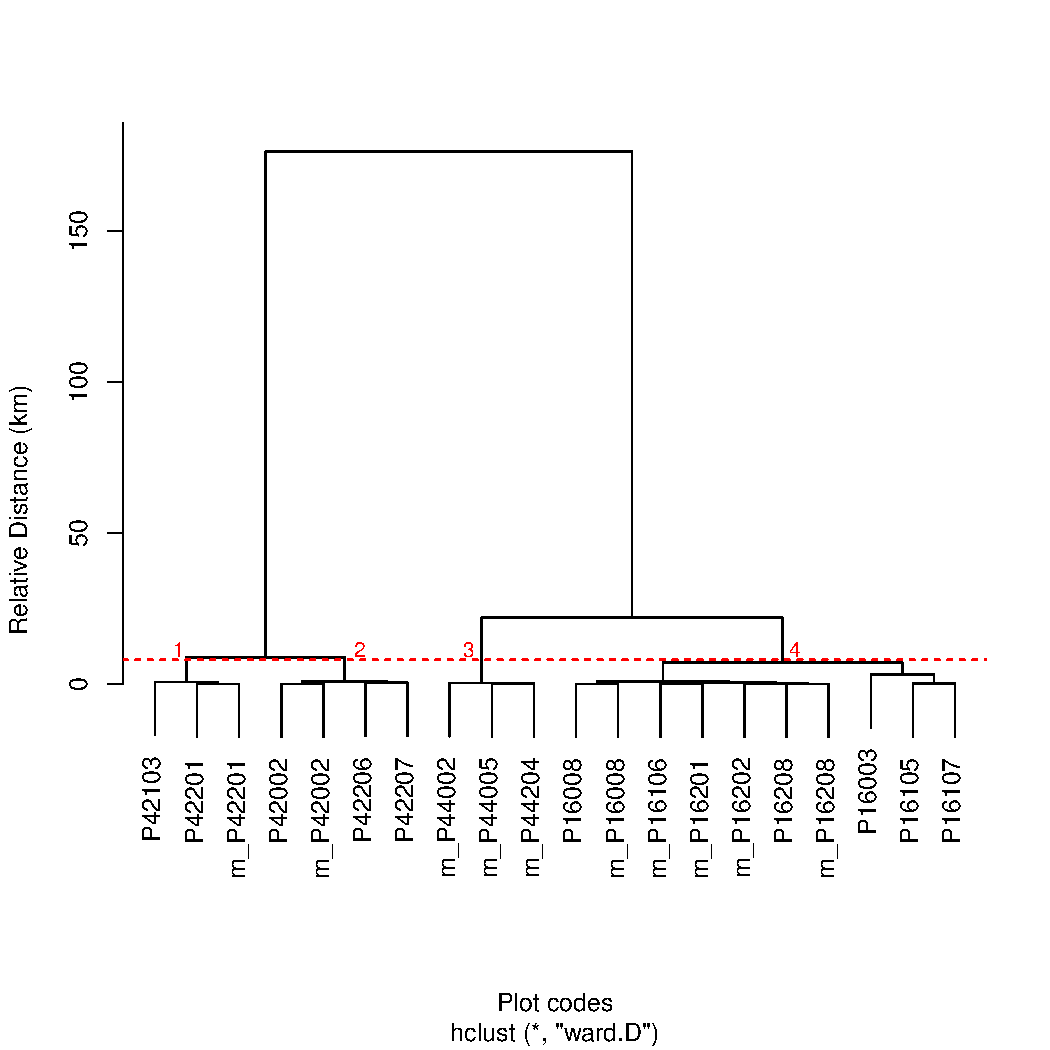
\includegraphics[scale=0.8,trim=20mm 0mm 20mm 0mm]{clust} 
\caption{Relative geographic closeness between sample plots. Plots with
  master series are indicated with m\_. Codes of sample plots begin with
  initial letter of the species (\textit{P. pinaster}); following with
  two digits in code indicating the province code: 42 corresponding to
  \textit{Soria} on Northern protion of \textit{Ebro} river basin, and
  16 being \textit{Cuenca} on Southern region of such a basin; last
  three digits in codes indicate individual number of the sample
  plot. Sample plots of master series have been indicated with the
  letter m\_. Black dashed line splits distance dendrogram in the two
  geographical portions of the river basin: North and South (distances
  $>$ 1500 km); and the red dashed line defines four groups used to
  statistically control (cross-dating) dendrochronological series
  (distances $<$ 80 km).}
\label{fig:clust} 
\end{figure}



\clearpage
%poner los lugares de isótopos puntos negros
\begin{figure}\centering
\includegraphics[scale=0.5,trim=20mm 0mm 20mm 0mm]{map_03} 
\caption{Study site. The green areas represent distribution of
  \textit{P. pinaster} along Spain. The orange points represent
  locations of tree-ring chronologies only}
\label{fig:map_03} 
\end{figure}

\clearpage
\begin{figure}\centering
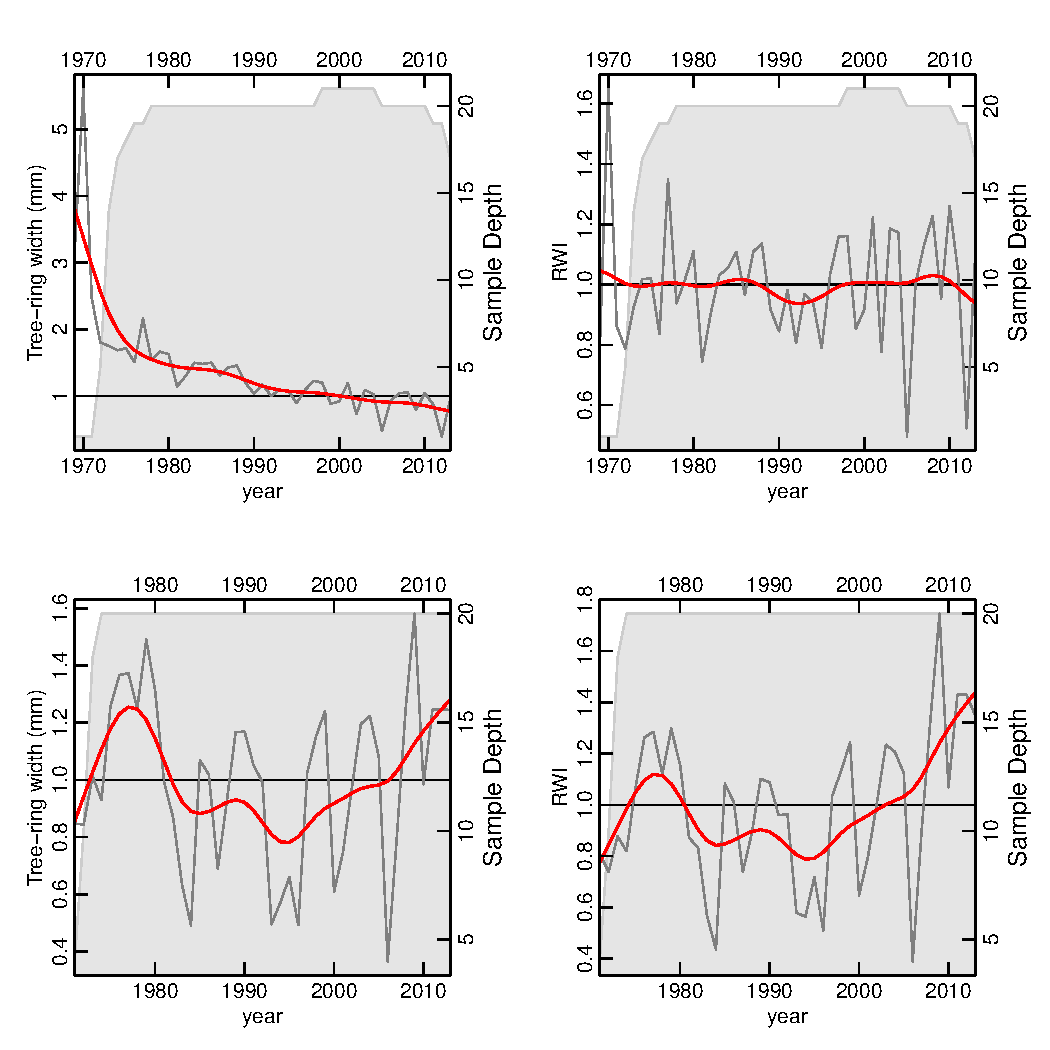
\includegraphics[scale=0.7,trim=20mm 0mm 20mm 0mm]{RWIs} 
\caption{Tree-ring-width chronologies of \textit{P. pinaster} trees
  growing on north (upper-panel plots) and east-central Spain
  (lower-panel plots). Trends in original chronologies (left-panel
  plots) are subtracted (right-panel plots). Gray lines indicate
  fluctuations, and red lines suggest average patterns. Sample depth
  is the number of series available in each year.}
\label{fig:RWIs} 
\end{figure}

\clearpage
\begin{figure}\centering
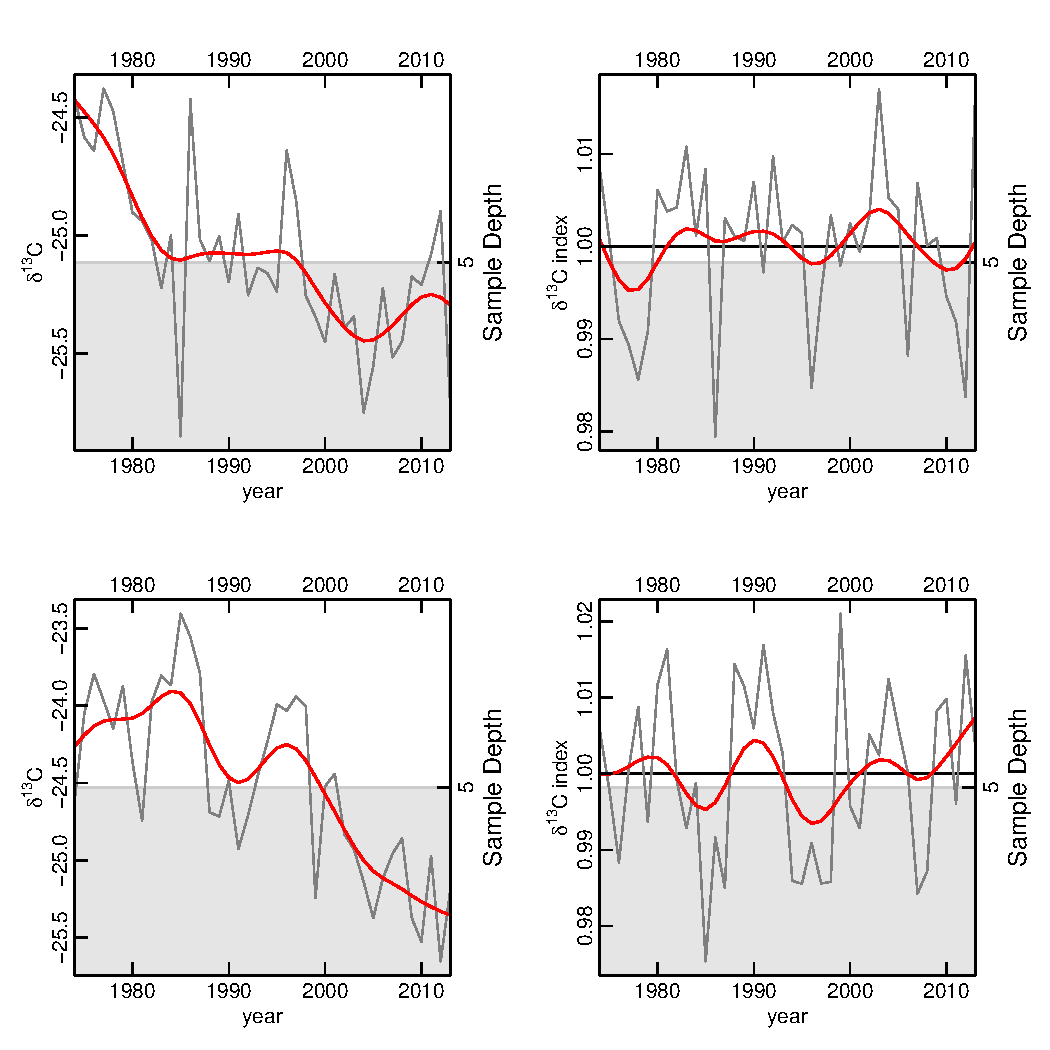
\includegraphics[scale=0.7,trim=20mm 0mm 20mm 0mm]{ideltas} 
\caption{Isotopic chronologies of \textit{P. pinaster} trees growing
  on north (upper-panel plots) and east-central Spain (lower-panel
  plots). Trends in original chronologies (left-panel plots) are
  subtracted (right-panel plots). Gray lines indicate fluctuations,
  and red lines suggest average patterns. Sample depth is the number
  of series available in each year.}
\label{fig:LWSC} 
\end{figure}

\clearpage
% obn: cambiar south by east-central Spain
\begin{landscape}
\begin{figure}
% \centering
\begin{minipage}[b]{0.8\textwidth}
\centering
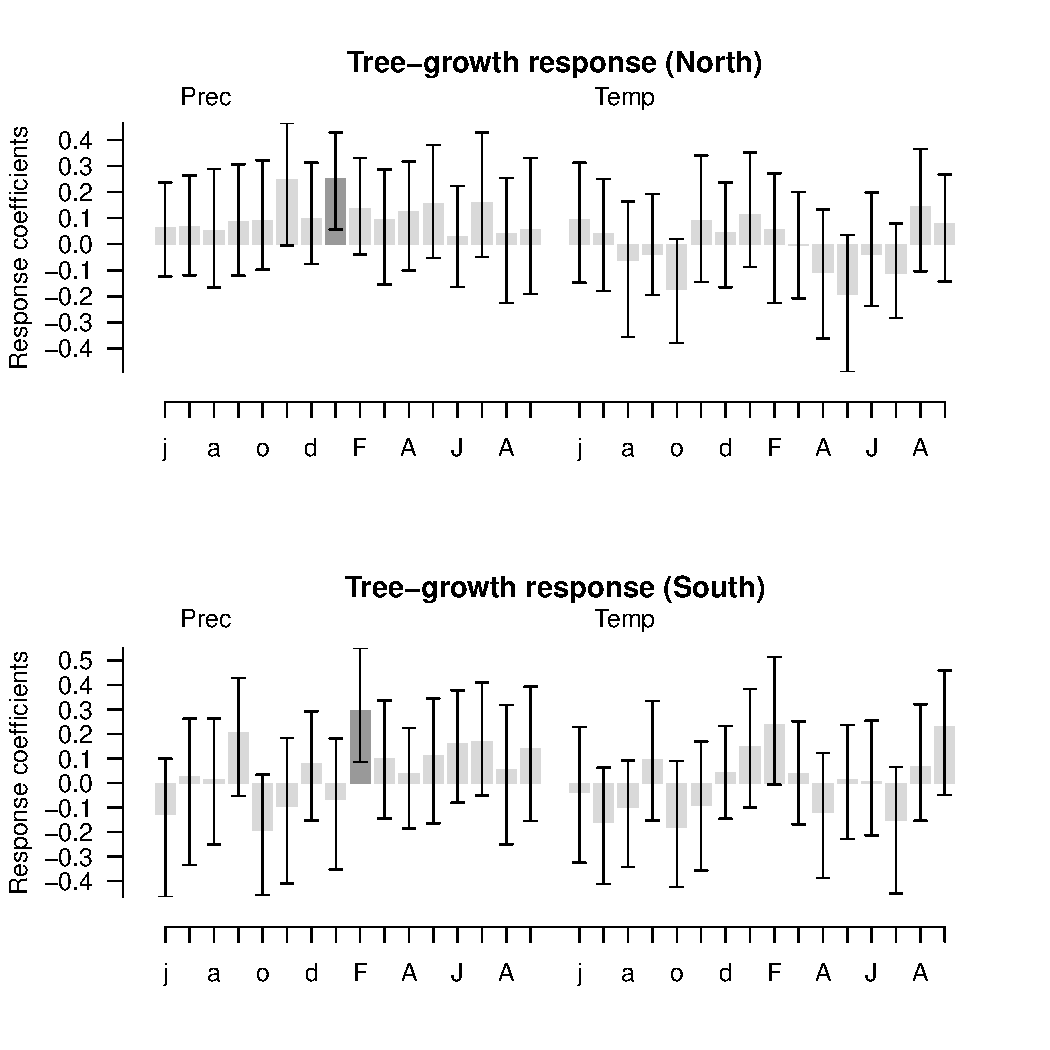
\includegraphics[width = \textwidth]{GrowthFunRes}
\end{minipage}
\begin{minipage}[b]{0.8\textwidth}
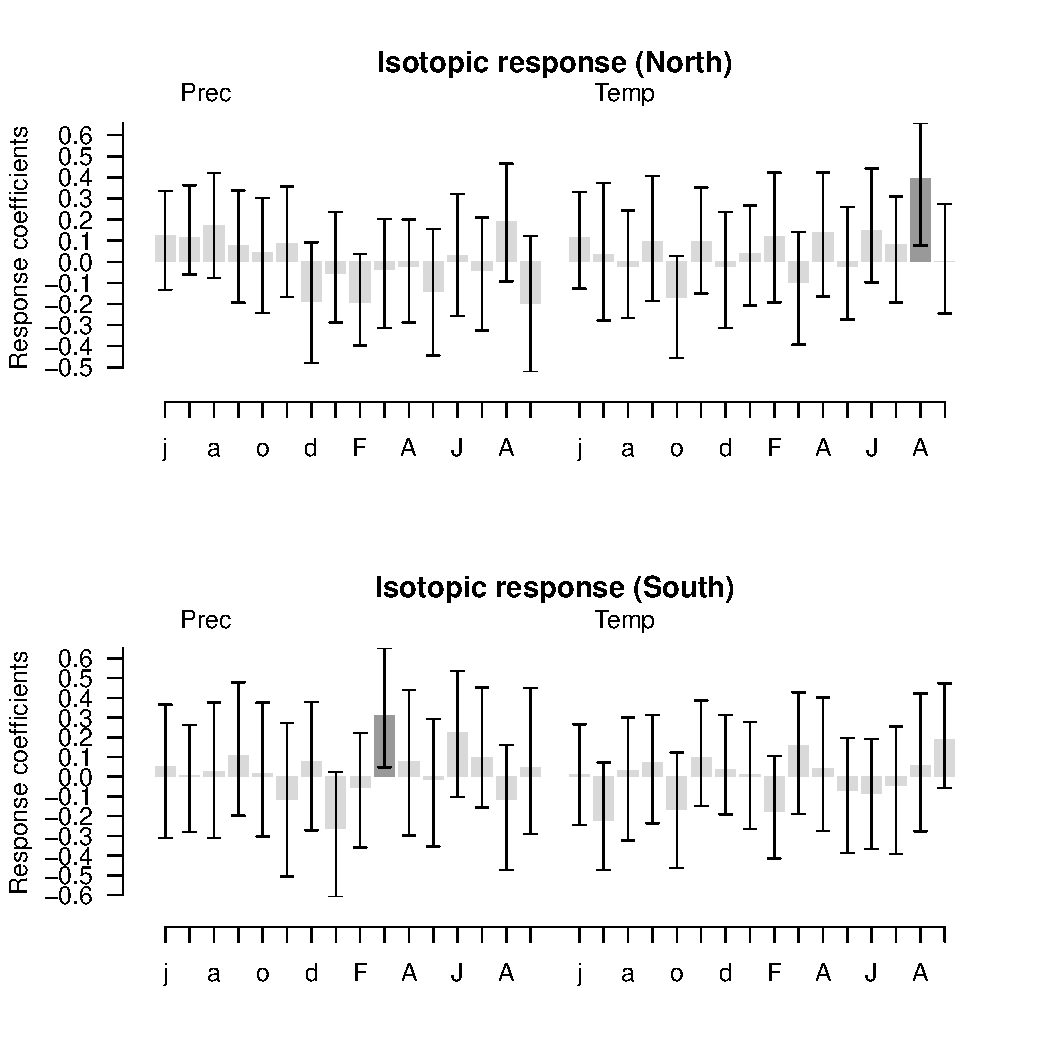
\includegraphics[width = \textwidth]{IsoFunRes}
\end{minipage}
\label{fig:FunRes}
\caption{Intra-annual response coefficients for precipitation and
  temperature for tree-ring and isotopic chronologies of
  \textit{P. pinaster}. The darker bars indicate signifficant
  coefficients ($P\le0.05$), and the lines represent $95\%$-confidence
  intervals.}
  \end{figure}
\end{landscape}

\clearpage
\begin{figure}
\centering
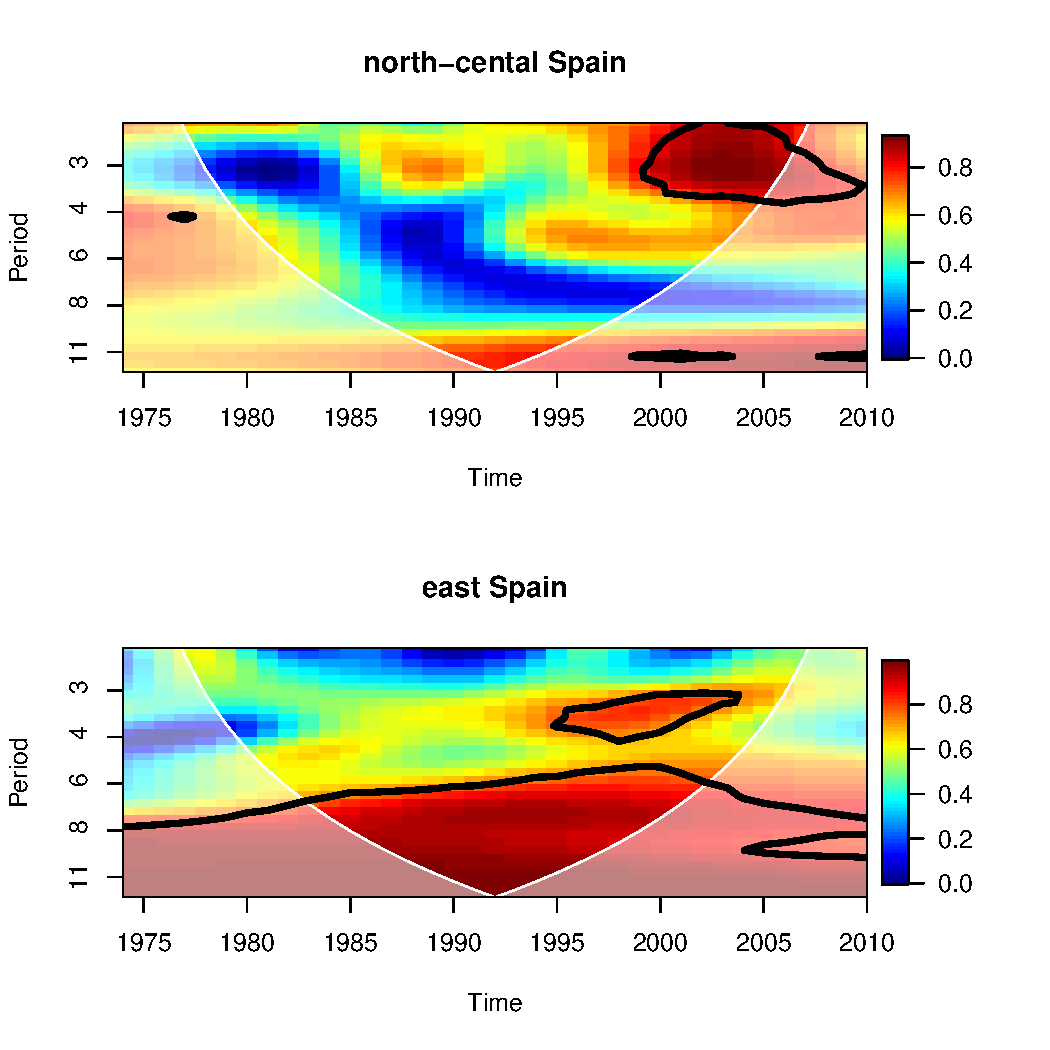
\includegraphics[scale=0.7,trim=20mm 0mm 20mm 0mm]{coherence1}
\label{fig:cohe}
\caption{Wavelet coherency between signals of tree-ring widths and
  standardized precipitation indexes. The colored scale indicate the
  correlation between the two time series.}
\end{figure}

% \clearpage
% \begin{figure}\centering
% 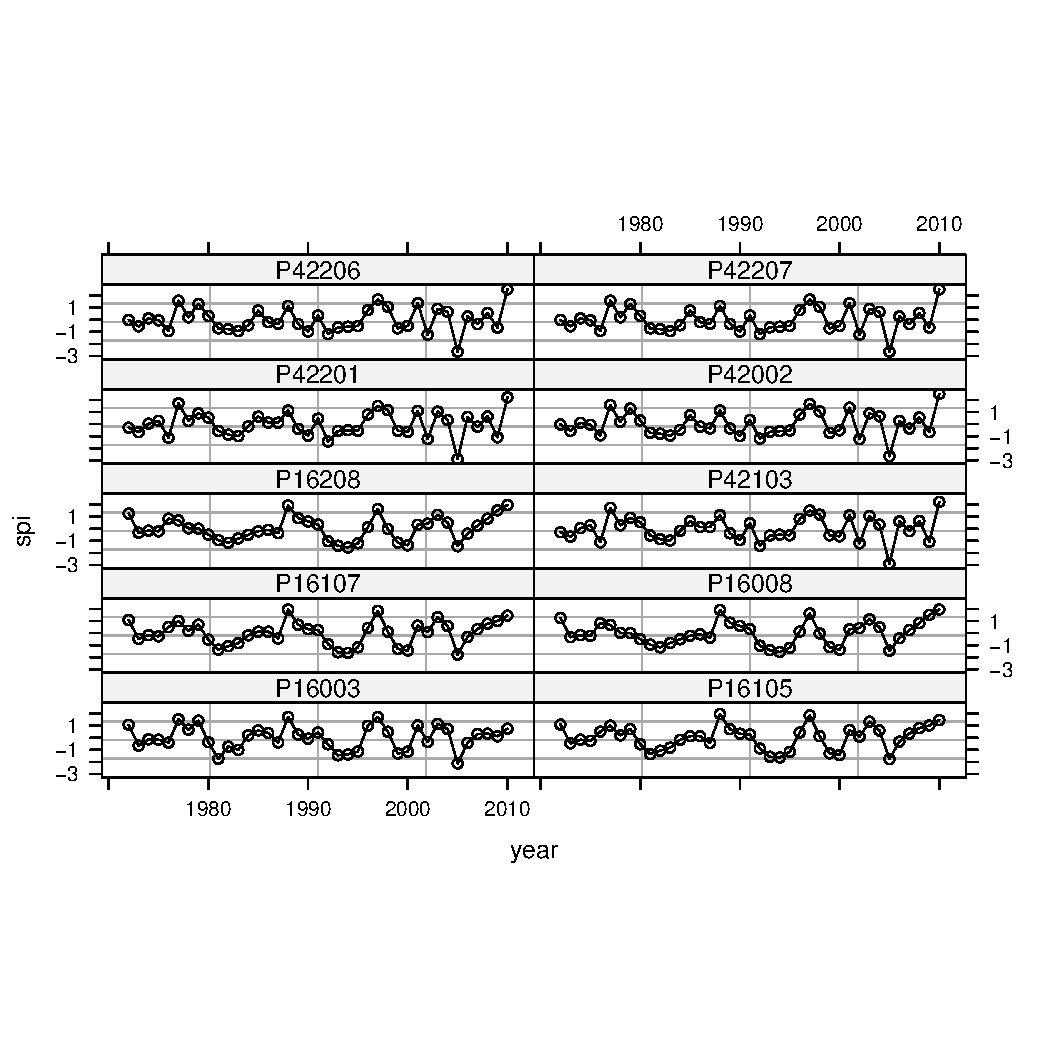
\includegraphics[scale=0.8,trim=20mm 0mm 20mm 0mm]{spis} 
% \caption{Series of standardized precipitation indexes (spi) on ten
%   sample plots of \textit{P. pinaster} located on Northern protion of
%   \textit{Ebro} river basin (42: \textit{Soria}) and on Southern
%   region of such a basin (16: \textit{Cuenca}). Panels are ordered
%   from plots with lower spi values (lower-left panel) to plots with
%   higher spi extremes (higher-right panel).See legend in Figure
%   \ref{fig:clust} for further explanation of both: codes and plot
%   locations.}
% \label{fig:spis} 
% \end{figure}

% \clearpage
% \begin{figure}\centering
% 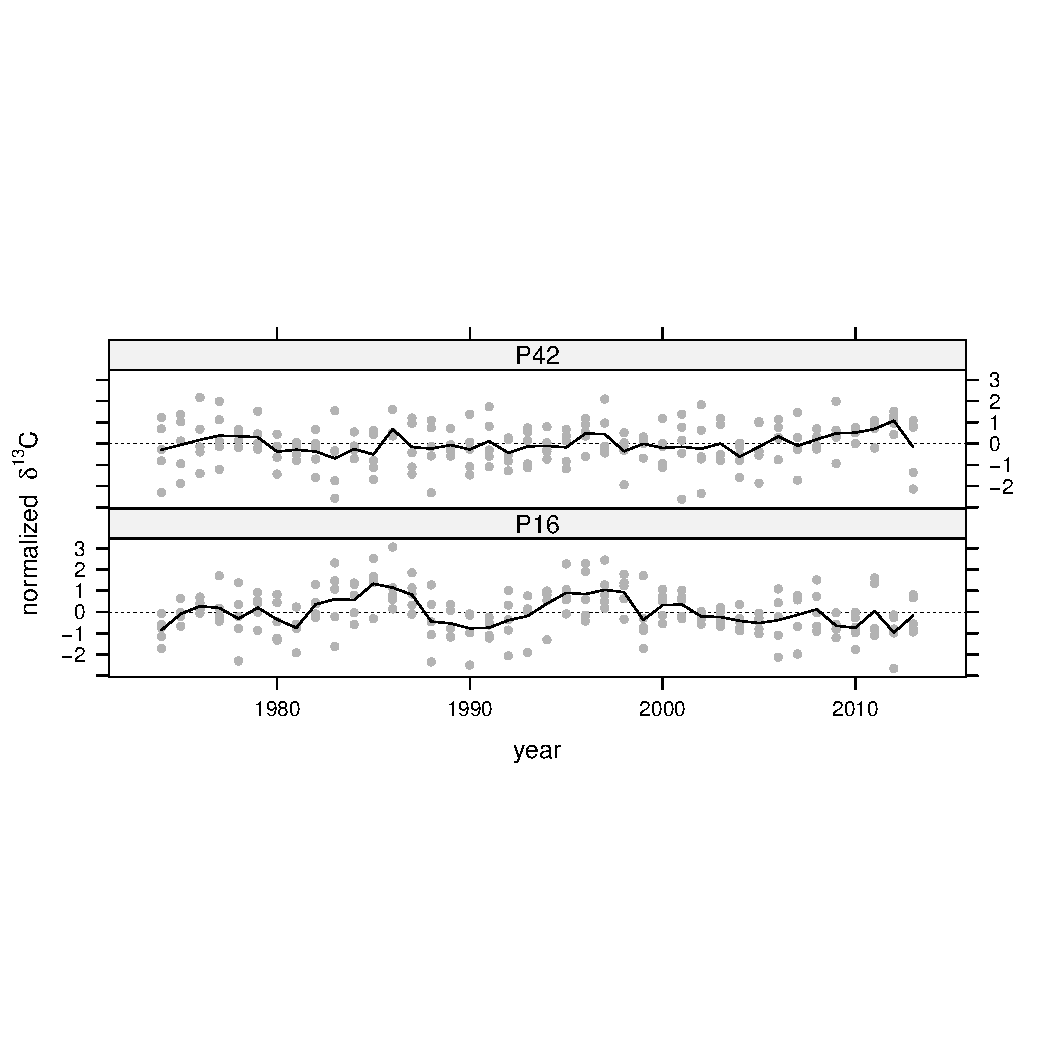
\includegraphics[scale=0.9,trim=20mm 0mm 20mm 0mm]{isoYr}
% \caption{Normalized $\delta^{13}$C of
%   \textit{P. pinaster} late-wood in trees growing on Northern Ebro basin
%   (P42) and Southern portion of the basin (P16), Spain}
% \label{fig:isoyr} 
% \end{figure}

 
% \clearpage
% \begin{figure}\centering
% 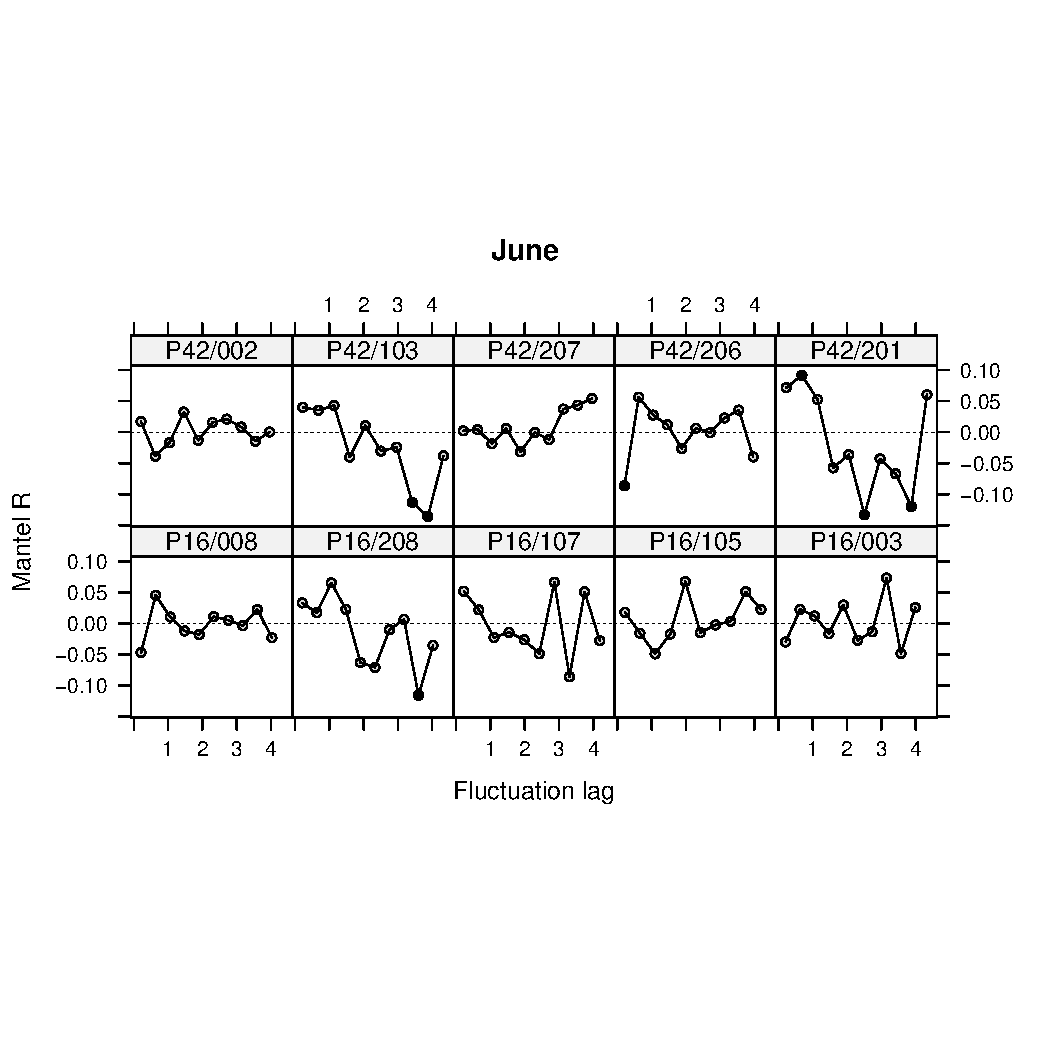
\includegraphics[scale=0.9,trim=20mm 0mm 20mm 0mm]{mflucJun} 
% \caption{Signatures between normalized $\delta^{13}$C of
%   \textit{P. pinaster} late-wood and precipitation indexes
%   (June) from 1974 to 2010. Signatures where computed with Multilevel
%   correlograms. The Fluctuation lags where computed with Sturdges'
%   rule. $10^4$ permutation texts where developed on compared
%   fluctuation-distance matrices.}
% \label{fig:signjun} 
% \end{figure}
% \begin{figure}\centering
% 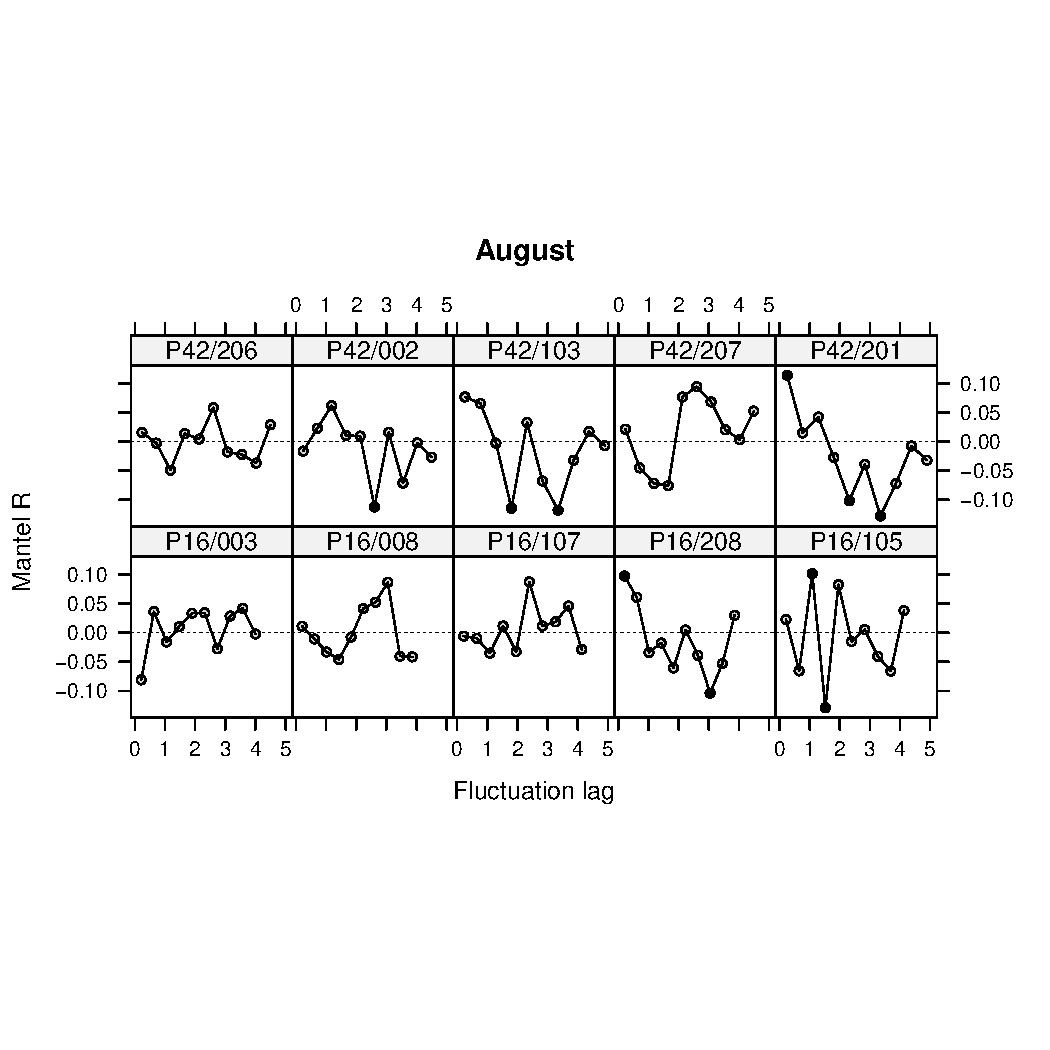
\includegraphics[scale=0.8,trim=20mm 0mm 20mm 0mm]{mflucAug} 
% \caption{Signatures between normalized $\delta^{13}$C of
%   \textit{P. pinaster} late-wood and precipitation indexes
%   (August) from 1974 to 2010. Signatures where computed with Multilevel
%   correlograms. The Fluctuation lags where computed with Sturdges'
%   rule. $10^4$ permutation texts where developed on compared
%   fluctuation-distance matrices.}
% \label{fig:sigaug} 
% \end{figure}

\end{document}
